\subsection{NDVI}
\textit{The following section is a slightly reworked version of a section from the pre-thesis master project~\cite{andrae2023}} 
%
\noindent
\begin{figure}[!htbp]
%\begin{wrapfigure}{r}{0.62\textwidth}
    \centering
    %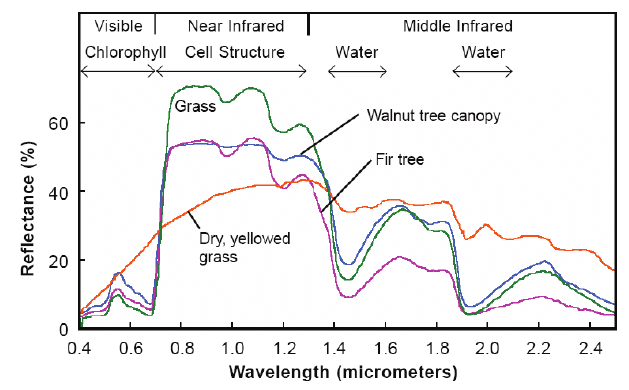
\includegraphics[width=0.60\textwidth]{img/Reflectance-spectra-of-different-types-of-green-vegetation-compared-to-a-spectral.png}
    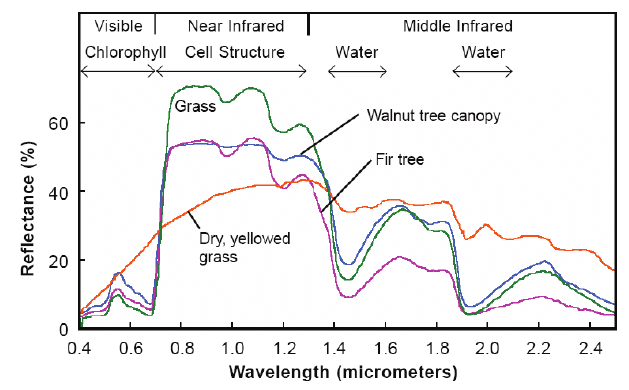
\includegraphics[width=0.5\textwidth]{img/Reflectance-spectra-of-different-types-of-green-vegetation-compared-to-a-spectral.png}
    \caption{Absorption spectrum of green vegetation\cite[Fig. 2]{Govender2007}\label{fig:absorbtionVeg}}
%\end{wrapfigure}
\end{figure}
The \gls{NDVI} is an widely used index using the difference of the red and near infrared bands to determine the amount of green vegetation. 
\begin{equation}
    NDVI = \frac{Red-NIR}{Red+NIR}
    \label{equ:ndvi}
\end{equation}
For Landsat 7 data channel 3 (red and orange: $630\ \text{nm} - 690 \text{nm}$) and channel 4 (near infrared $780\ \text{nm} - 900 \text{nm}$) are used for \gls{NDVI} calculation.  
For Landsat 8 and 9 data, channel 4 (red $640\ \text{nm} - 670\ \text{nm}$) and channel 5 (near infrared $850\ \text{nm} - 880\ \text{nm}$) where used.
As shown in \cref{fig:absorbtionVeg} healthy plants reflect near infrared and there is a sharp rise in reflectance between the two used channels at around $700\ \text{nm}$. 
%
This index is used for emissivity estimation for Land Surface Temperature calculation see \cref{equ:toa}, correlation with heat islands (since there is a negative correlation between those two values, due to the latent heat of evaporation reducing surface temperature at higher vegetation areas).
\begin{figure}[!htbp]
    \centering
    \begin{subfigure}{0.45\textwidth}
    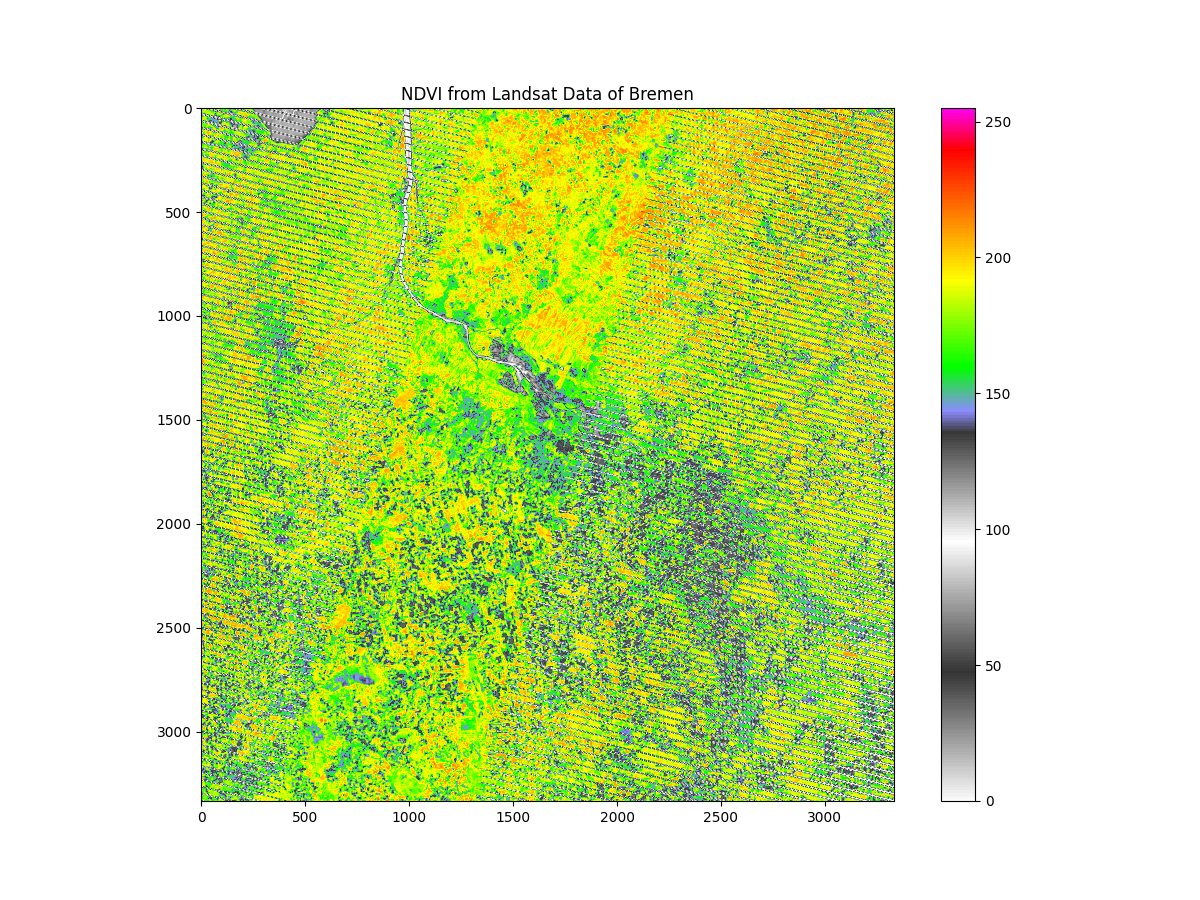
\includegraphics[width=\textwidth]{img/NDVI_LE07_L1TP_196023_20190723_20200825_02_T1__Bremen.png}
    \subcaption{NDVI of Bremen (Bands 5 and 6) using Landsat 7 data on 2019--07--23}
    \end{subfigure}
    \begin{subfigure}{0.45\textwidth}
    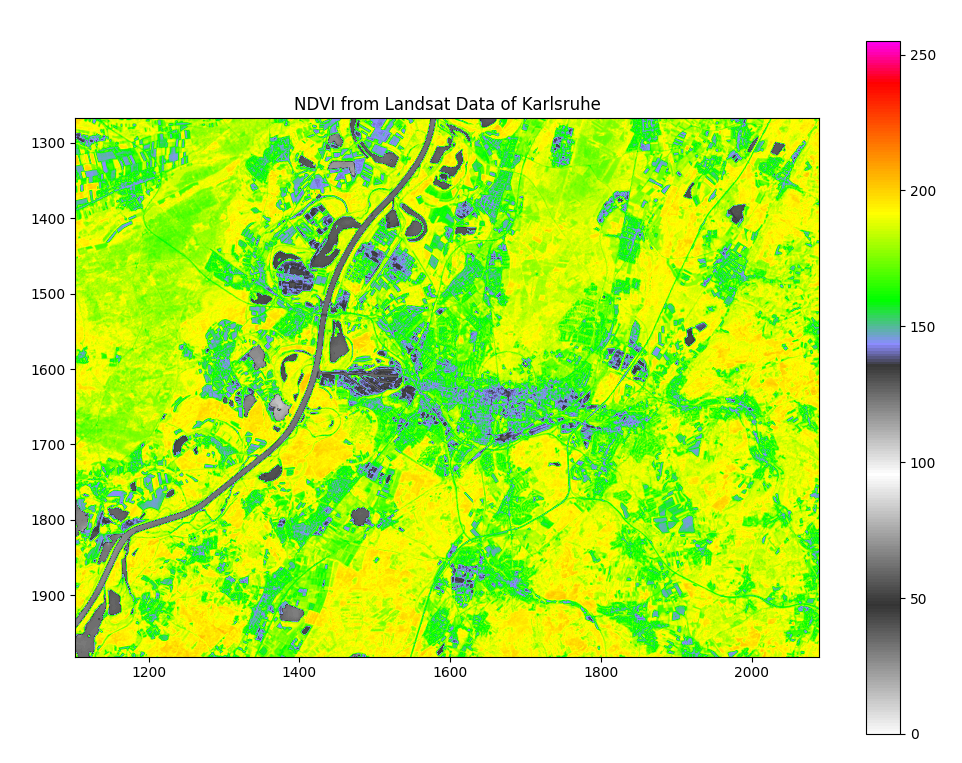
\includegraphics[width=\textwidth]{img/KarlsruheNDVI_Landsat8.png} 
    \subcaption{NDVI of Karlruhe (Bands 4 and 5) using Landsat 8 data on 2023--06--07}
    \end{subfigure}
    \caption{NDVI Images from the different satellites\label{fig:ndvi}}
\end{figure}
\subsubsection{NDVI Colormap}\label{sec:colormap}
When using a classical heat map with a color gradient from colder to warmer colors or a diverging color map (see \cref{fig:ndviPhoenixAzBad}), details of the image get lost and it is hard to distinguish plant heath, build up and vegetated areas and the difference between small \gls{NDVI} changes.
To aid an intuitive understanding a specially created colormap can be used. 
The color map was adapted for use in python from work of \texttt{public lab}\cite{ndviCmap} where it was developed in an attempt to create color-blind friendly \gls{NDVI} color maps.
Values below 0.2 are areas with no vegetation.
The color map used in \cref{fig:ndviPhoenixAz} uses a gradient of gray with a ``black-white-black
white'' transition to allow higher dynamic range for non vegetation areas.
For areas with an \gls{NDVI} $<$ 0.2 blue is used. Green values are low or unhealthy green vegetation or mixed use pixels. 
Orange and red values correspond to thicker vegetation e.g.~forests, parks or green fields. 
%
Comparing \cref{fig:ndviPhoenixAz}  and \cref{fig:ndviPhoenixAzBad} where most of the desert surrounding the city has no green vegetation and the parts covered in vegetation can be clearly distinguished from the arid desert regions.
Still the surface roughness can be seen quite well due to the gray scale gradient in the $<$ 0.2 \gls{NDVI} range.  
%
\begin{figure}[htbp]
 \centering
    \begin{subfigure}{0.46\textwidth}
    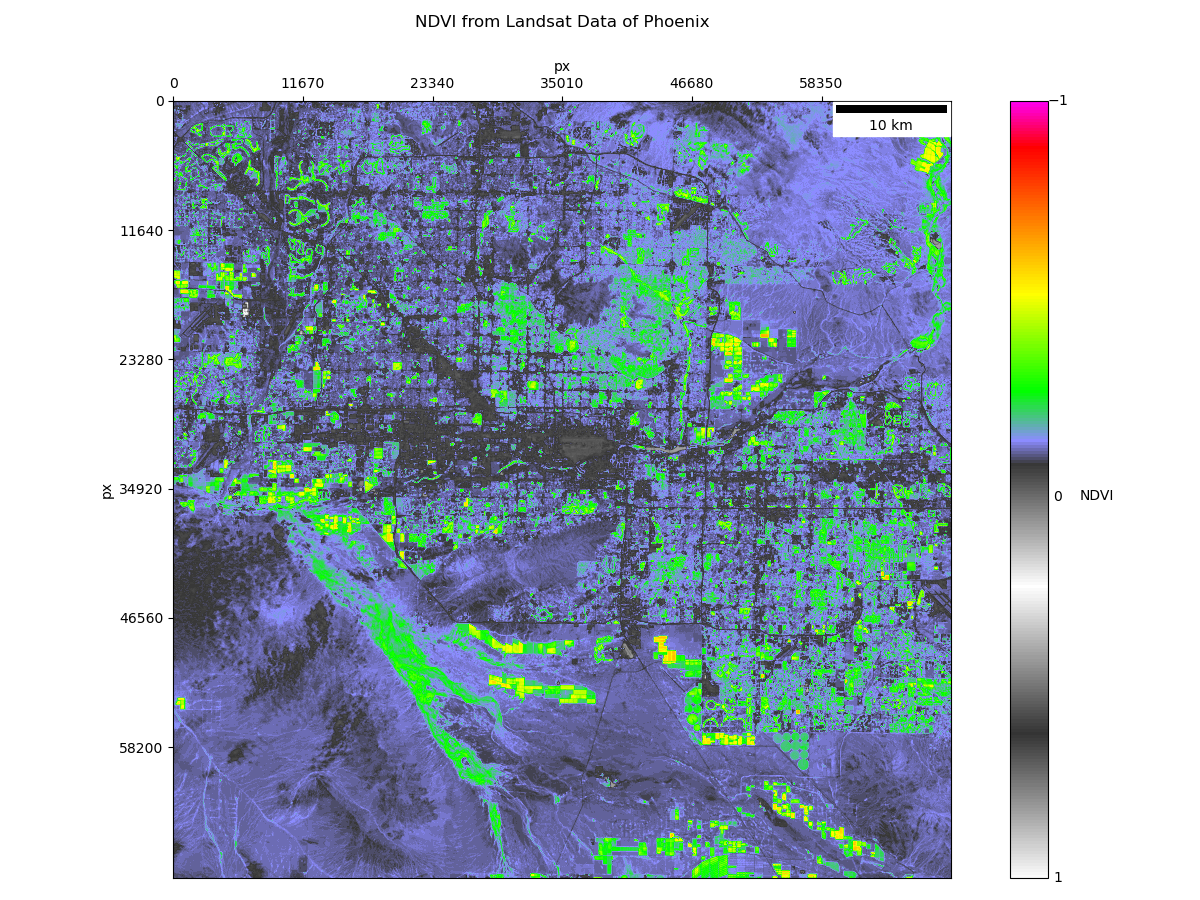
\includegraphics[width=\textwidth]{img/NDVI from Landsat Data of Phoenix.png} 
    \subcaption{NDVI Image of Phoenix with the  VGYRM color map\label{fig:ndviPhoenixAz}}
    \end{subfigure}
    \begin{subfigure}{0.46\textwidth}
    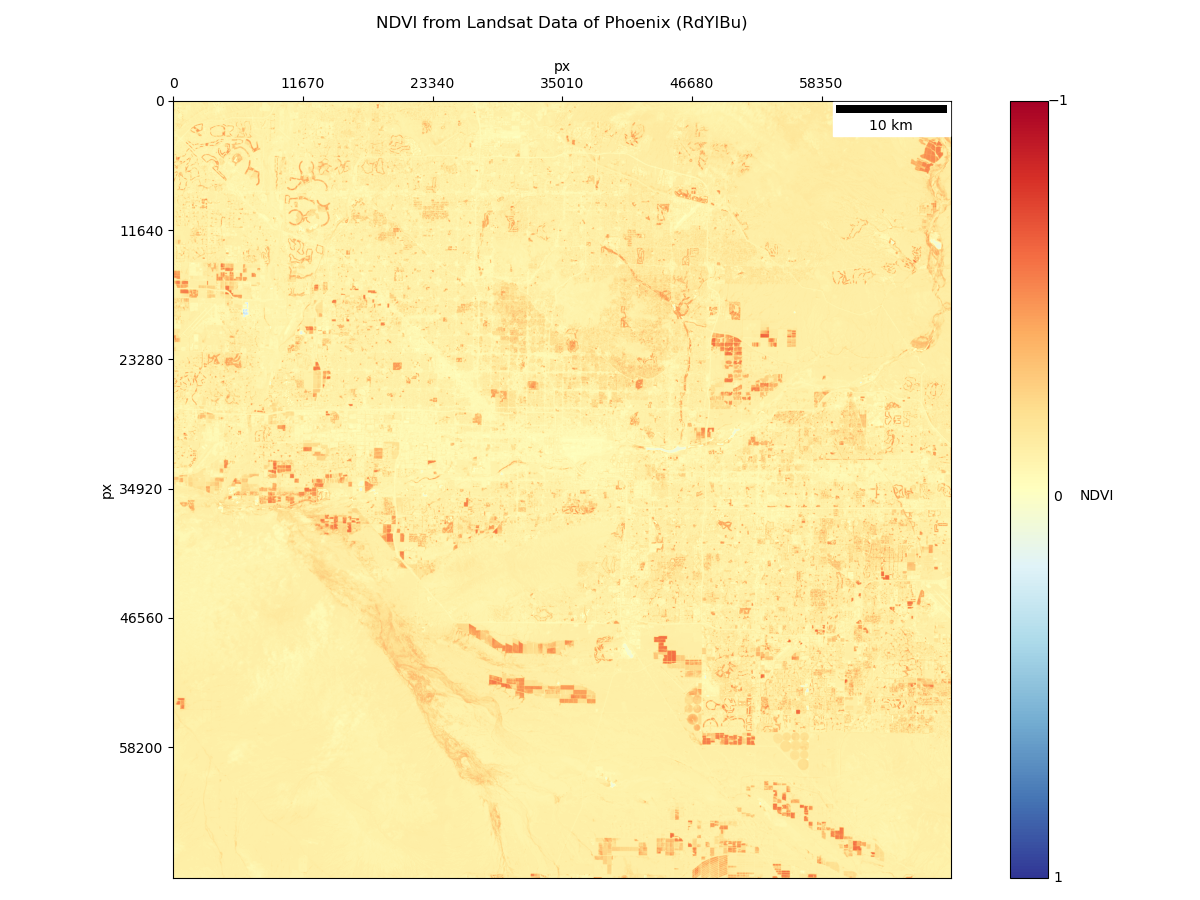
\includegraphics[width=\textwidth]{img/NDVI from Landsat Data of Phoenix (RdYlBu).png} 
    \subcaption{NDVI Image of Phoenix with a RdYlBu gradient color map\label{fig:ndviPhoenixAzBad}}
    \end{subfigure}
    \caption{Different color maps used show the better ability to differentiate between green vegetation and desert and buildings within Phoenix\label{fig:ndvicomp}}
\end{figure}
